% Information Processing & Management (IP&MC 2026) submission.
% Elsevier elsarticle class, single-column review format, Vancouver-numbered refs.
% Compile: pdflatex main; pdflatex main  (manual thebibliography, no bibtex pass needed)
\documentclass[review,12pt]{elsarticle}

\usepackage{graphicx}
\graphicspath{{figures/}}
\usepackage{booktabs}
\usepackage{multirow}
\usepackage{amsmath}
\usepackage{amssymb}
\usepackage{algorithm}
\usepackage{algpseudocode}
\usepackage[colorlinks=true,linkcolor=blue,citecolor=blue,urlcolor=blue]{hyperref}

\journal{Information Processing \& Management}

\begin{document}

\begin{frontmatter}

\title{Federated Retraction Prediction: Scaling Scientific-Integrity
Screening Across Publisher Silos}

\author[inst1]{Muhammad Ahmad\corref{cor1}}
\ead{ahmad.stmu@gmail.com}
\author[inst2]{Muhammad Tanvir Afzal}
\ead{tanvir.afzal@gisma.com}
\cortext[cor1]{Corresponding author}
\affiliation[inst1]{organization={Independent Researcher},
            country={Pakistan}}
\affiliation[inst2]{organization={Gisma University of Applied Sciences GmbH},
            city={Potsdam},
            country={Germany}}

\begin{abstract}
Retractions of scientific publications are growing rapidly, straining the
integrity of the scholarly record, yet automated screening remains limited by
two structural constraints: prior work relies on small hand-curated corpora,
and the strongest predictive signals (full text, citation contexts, and
editorial metadata) are fragmented across publishers that cannot legally pool
their data. We cast large-scale retraction prediction as a \emph{cross-silo
federated learning} problem. From the Retraction Watch database enriched with
OpenAlex metadata we construct a corpus of 138{,}537 articles (37{,}648
retracted; publisher- and year-matched controls), 180$\times$ larger than the
largest corpus in prior retraction-prediction studies. We simulate realistic
publisher and discipline silos, naturally non-IID in size, era, and topical
composition, and benchmark local-only and centralized training against FedAvg
and FedProx, adding a differentially private variant. Federated training
attains 92\% of the AUPRC of an identical centrally trained model (0.558 vs.\
0.609) while improving 77\% over the silo-local status quo (0.315), and remains
stable as the consortium grows from 5 to 20 silos. Cross-corpus experiments
against the hand-curated benchmark of prior work show that models trained on
hundreds of curated articles collapse to chance on the open corpus, that
abstract-level features alone reduce prior reported accuracy from 0.88 to
chance (quantifying how much signal is locked in paywalled full text), and that
linguistic features transfer across domains while metadata features do not.
Together these results position federated learning as the deployment path for
retraction screening at the scale of the scientific record.
\end{abstract}

\begin{keyword}
Retraction prediction \sep Federated learning \sep Scientific integrity \sep
Digital libraries \sep Scholarly communication \sep Differential privacy
\end{keyword}

\end{frontmatter}

%% ====================================================================
\section{Introduction}
\label{sec:intro}
The retraction of scientific publications has grown from isolated incidents to
a systemic phenomenon: the Retraction Watch database now records more than
71{,}000 retraction events, with over 15{,}000 in 2024
alone~\cite{ref_rw,ref_vannoorden}. Because a retraction takes up to three
years on average to be issued, flawed results continue to be cited, reused,
and built upon long after problems are first suspected~\cite{ref_usman_tpdl23}.
For digital libraries, indexing services, and publishers, the ability to flag
at-risk articles early is therefore a core problem of maintaining the integrity
of the scholarly information ecosystem. A line of recent work by Usman and
Balke~\cite{ref_usman_tpdl23,ref_usman_tpdl24,ref_usman_dasfaa25,ref_usman_websci25}
demonstrated that retraction is predictable from how articles are written and
cited: readability and certainty of full-text sections separate retracted from
non-retracted articles with 0.88 accuracy~\cite{ref_usman_websci25}, and
citation sentences anticipate retraction cascades~\cite{ref_usman_tpdl24}.

Yet this evidence was obtained on corpora of a few hundred hand-curated
articles, and its authors note that re-evaluating the complete scientific
literature with such methods is infeasible. We argue the obstacle is
structural rather than methodological. The strongest features require full
text and editorial context, which are held by \emph{different publishers} and
cannot be pooled for legal and commercial reasons. Any deployable system must
therefore learn \emph{across} data silos without moving the data.

\paragraph{Problem statement.}
Let $\mathcal{P} = \{P_1,\dots,P_K\}$ be $K$ data owners (publishers or
disciplinary databases). Each holds a private dataset
$D_k = \{(\mathbf{x}_i, y_i)\}_{i=1}^{n_k}$ of articles with features
$\mathbf{x}_i \in \mathbb{R}^d$ and retraction labels $y_i \in \{0,1\}$,
where the $D_k$ differ in size, feature distribution, and label prevalence
(statistical heterogeneity). The goal is to learn a global predictor
$f_\theta$ minimizing
\begin{equation}
\min_\theta \; F(\theta) \;=\; \sum_{k=1}^{K} \frac{n_k}{n}\, F_k(\theta),
\qquad
F_k(\theta) = \frac{1}{n_k} \sum_{(\mathbf{x},y)\in D_k}
\ell\bigl(f_\theta(\mathbf{x}),y\bigr),
\label{eq:objective}
\end{equation}
subject to the constraint that raw records never leave their silo:
\begin{equation}
D_k \;\text{is accessed only by}\; P_k, \qquad
\text{only model parameters}\;\theta\;\text{are exchanged}.
\label{eq:constraint}
\end{equation}

\paragraph{Contributions.}
(1)~The first formulation of retraction prediction as cross-silo federated
learning, with an open, reproducible benchmark of 138{,}537 articles across
naturally non-IID publisher and discipline silos, 180$\times$ larger than
prior retraction-prediction corpora.
(2)~A systematic comparison of local-only, centralized, and federated
training (FedAvg, FedProx), showing federation recovers 92\% of centralized
AUPRC and improves 77\% over the silo-local status quo, robustly across two
silo definitions, consortium sizes 5--20, and a temporal split.
(3)~A differential-privacy analysis quantifying the utility cost of protecting
individual records in the federated setting.
(4)~Cross-corpus experiments against the benchmark of
\cite{ref_usman_websci25} that measure, for the first time, how much
retraction signal is locked in paywalled full text, and reveal that linguistic
features transfer across domains while metadata features do not.

\section{Related Work}
\label{sec:related}
\paragraph{Retraction analysis and prediction.}
Usman and Balke introduced citation-intention analysis as a quality-control
mechanism~\cite{ref_usman_tpdl23}, traced retraction cascades to identify
not-yet-retracted but suspicious articles~\cite{ref_usman_tpdl24}, defined
\emph{concerning citations} as early self-correction
signals~\cite{ref_usman_dasfaa25}, and showed that section-level readability
and certainty separate methodology-error retractions from matched controls
with Random Forests at 0.88 accuracy, outperforming
BioBERT~\cite{ref_usman_websci25}. Within this journal, bibliometric studies
similarly identify interpretable metadata correlates of
retraction~\cite{ref_bibliometric}.
\textbf{Limitation.} All rely on centralized corpora of at most a few
thousand hand-curated instances; the features that perform best require full
text that no single party can obtain at scale.

\paragraph{Federated learning.}
FedAvg~\cite{ref_fedavg} established communication-efficient averaging of
locally trained models; FedProx~\cite{ref_fedprox} adds a proximal term for
heterogeneous clients; a broad survey is given in~\cite{ref_kairouz}.
Differentially private aggregation clips and noises client
updates~\cite{ref_dpfl}. Cross-silo FL is deployed in domains such as
healthcare and finance where data sharing is legally constrained.
\textbf{Limitation.} FL has not previously been applied to scientific-integrity
screening, and scholarly-domain benchmarks with \emph{naturally} non-IID
silos are lacking; most FL benchmarks impose synthetic Dirichlet splits on
image corpora.

\section{Federated Retraction Prediction}
\label{sec:method}

\subsection{Architecture}
Figure~\ref{fig:arch} shows the system. Each publisher runs local feature
extraction and local training on its private archive; a coordination server
aggregates parameter updates into a global model that is redistributed each
round. No article, label, or feature vector crosses a silo boundary,
satisfying constraint~\eqref{eq:constraint}.

\begin{figure}[t]
\centering
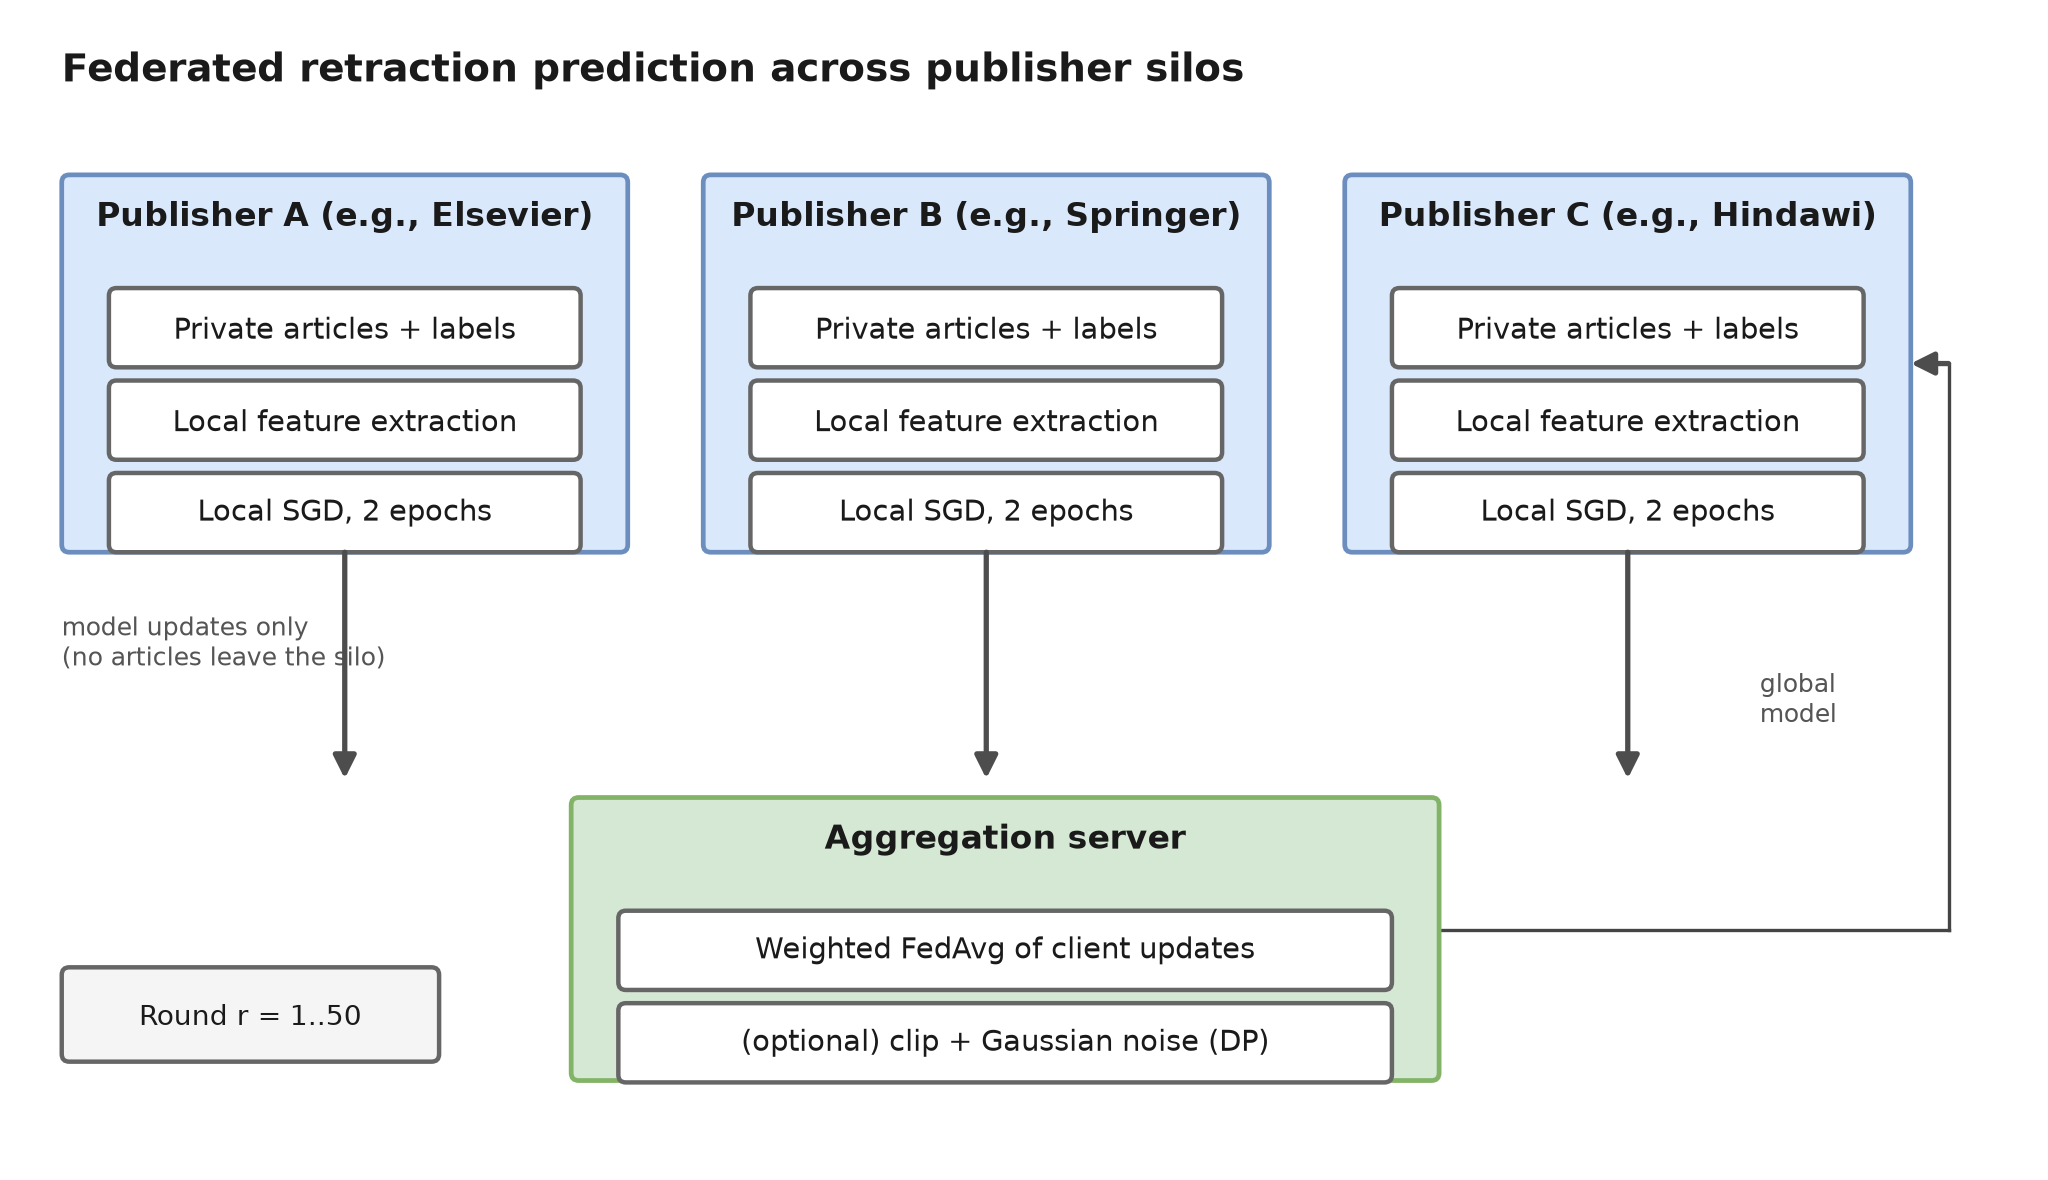
\includegraphics[width=\textwidth]{architecture.png}
\caption{Federated retraction prediction. Publishers train locally on private
articles; only model updates are aggregated (optionally clipped and noised for
differential privacy), and the global model is redistributed.}
\label{fig:arch}
\end{figure}

\subsection{Training procedure}
We use the small multilayer perceptron $f_\theta$ (two hidden layers, 64 and
32 units, ReLU, dropout 0.2) for all federated experiments, so that federated
and centralized results are architecture-identical. Local training minimizes
class-weighted binary cross-entropy
\begin{equation}
\ell(\hat y, y) = -\,w_1\, y \log \sigma(\hat y) - (1-y)\log\bigl(1-\sigma(\hat y)\bigr),
\qquad w_1 = \tfrac{n_k^{(0)}}{n_k^{(1)}},
\label{eq:loss}
\end{equation}
with $n_k^{(c)}$ the count of class $c$ in silo $k$. FedProx adds
$\frac{\mu}{2}\lVert\theta-\theta^{(r)}\rVert^2$ to \eqref{eq:loss}.
Algorithm~\ref{alg:fl} summarizes one training run, including the optional
differentially private aggregation: each client's update is clipped to $L_2$
norm $C$ and Gaussian noise $\mathcal{N}(0, \sigma^2C^2/K)$ is added to the
average~\cite{ref_dpfl}; privacy is accounted over rounds with
R\'enyi-DP composition.

\begin{algorithm}[t]
\caption{DP-enabled cross-silo FedAvg for retraction prediction}
\label{alg:fl}
\begin{algorithmic}[1]
\State \textbf{input} silos $D_1,\dots,D_K$; rounds $R$; local epochs $E$;
clip $C$; noise $\sigma$
\State server initializes $\theta^{(0)}$
\For{$r = 1,\dots,R$}
  \For{each silo $k = 1,\dots,K$ \textbf{in parallel}}
    \State $\theta_k \gets$ \Call{LocalSGD}{$\theta^{(r-1)}, D_k, E$}
      \Comment{minimizes \eqref{eq:loss}; data stays in silo}
    \State $\Delta_k \gets \theta_k - \theta^{(r-1)}$;\quad
      $\Delta_k \gets \Delta_k \cdot \min\bigl(1, C/\lVert\Delta_k\rVert_2\bigr)$
  \EndFor
  \State $\bar\Delta \gets \frac{1}{K}\sum_k \Delta_k
    + \mathcal{N}\!\bigl(0,\, \sigma^2 C^2 / K\bigr)$
    \Comment{$\sigma{=}0$ recovers FedAvg}
  \State $\theta^{(r)} \gets \theta^{(r-1)} + \bar\Delta$
\EndFor
\State \Return $\theta^{(R)}$
\end{algorithmic}
\end{algorithm}

\subsection{Evaluation metrics}
With retracted articles a minority class, accuracy is uninformative. We report
the area under the precision--recall curve (AUPRC) as the primary metric,
\begin{equation}
\mathrm{AUPRC} = \int_0^1 \mathrm{Prec}\bigl(\mathrm{Rec}^{-1}(t)\bigr)\,dt,
\label{eq:auprc}
\end{equation}
whose random baseline equals the positive rate ($\approx 0.27$ on our corpus),
together with ROC-AUC and recall at 5\% false-positive rate
(R@5\%FPR), the fraction of future retractions caught when wrongly flagging
only 5\% of legitimate articles, the regime of an editorial pre-screening
tool. All results are means $\pm$ standard deviation over three seeds.

\section{A 138K-Article Federated Benchmark}
\label{sec:data}

\paragraph{Corpus construction.}
Positives are all Retraction Watch~\cite{ref_rw} research articles with a
resolvable DOI whose record nature is \emph{Retraction} (37{,}648 after
filtering). Each is enriched via the OpenAlex API~\cite{ref_openalex} with
authorship, venue, citation, and abstract metadata. Controls are sampled at
3:1 from OpenAlex among never-retracted articles of the \emph{same publisher
and publication year} (cells with fewer than five positives are dropped),
yielding 100{,}889 controls and 138{,}537 articles in total. Matching prevents
the classifier from exploiting publisher- or era-priors instead of
article-level signals.

\paragraph{Features.}
Each article is represented by $d{=}15$ features in two families, chosen to
mirror the signal types validated in prior
work~\cite{ref_usman_websci25,ref_usman_tpdl24}:
\emph{metadata} (author count, country count, international collaboration,
reference count, total citations, citations within two years of publication,
publication year, open-access flag) and \emph{abstract linguistics}
(Flesch reading ease, Flesch--Kincaid grade, Gunning--Fog, SMOG, abstract
length, hedging ratio, certainty ratio~\cite{ref_flesch,ref_kincaid}). In a
real deployment each publisher would additionally compute full-text features
locally; these are exactly the signals shown to be strongest in prior work and
inaccessible centrally; our public-metadata features are thus a conservative
lower bound on federated performance.

\paragraph{Silos.}
Articles are partitioned into $K{=}10$ silos by publisher (Table~\ref{tab:silos})
and, alternatively, by OpenAlex discipline. Silos differ strongly in size
(2{,}815--31{,}024 test$+$train articles), median era (2016--2022), and
composition. This is \emph{natural} statistical heterogeneity, in contrast to the
synthetic Dirichlet splits common in FL benchmarks.

\begin{table}[t]
\centering
\caption{Publisher silos (10-silo partition). Retraction rate is
$\approx$25\% by matched design; Hindawi exceeds it where control
sampling saturated.}
\label{tab:silos}
\small
\begin{tabular}{@{}lrrrr@{}}
\toprule
Silo & Articles & Retracted & Retr.\ rate & Median year \\
\midrule
Other (aggregated tail) & 31{,}024 & 8{,}007 & 0.258 & 2018 \\
Hindawi & 27{,}696 & 9{,}277 & 0.335 & 2022 \\
Elsevier & 21{,}221 & 5{,}722 & 0.270 & 2017 \\
Springer & 19{,}730 & 4{,}930 & 0.250 & 2020 \\
Wiley & 13{,}372 & 3{,}340 & 0.250 & 2020 \\
IOS Press & 8{,}320 & 2{,}080 & 0.250 & 2022 \\
PLOS & 4{,}960 & 1{,}240 & 0.250 & 2016 \\
SAGE & 4{,}772 & 1{,}193 & 0.250 & 2019 \\
Taylor \& Francis & 4{,}627 & 1{,}156 & 0.250 & 2018 \\
Spandidos & 2{,}815 & 703 & 0.250 & 2017 \\
\bottomrule
\end{tabular}
\end{table}

\section{Experiments}
\label{sec:experiments}
We evaluate on a stratified 20\% held-out test set shared by all training
regimes. \emph{Local-only} trains one model per silo and averages test
performance (the current deployable reality); \emph{centralized} pools all
data (the legally unattainable ideal; logistic regression, Random
Forest~\cite{ref_usman_websci25}-style, XGBoost, and the MLP);
\emph{federated} trains the MLP with Algorithm~\ref{alg:fl}
($R{=}50$, $E{=}2$, SGD with momentum 0.9, learning rate 0.05, $\mu{=}0.01$).

\subsection{Main result: federation closes the silo gap}
\label{sec:main}
Table~\ref{tab:main} and Fig.~\ref{fig:main} give the central result.
Local-only training barely beats the random baseline (AUPRC 0.315 vs.\ 0.27):
individual publishers, however large, cannot learn the global phenomenology of
retraction. FedAvg reaches 0.558: \textbf{92\% of the architecture-identical
centralized MLP} (0.609) and a \textbf{77\% improvement over the status quo},
with FedProx statistically indistinguishable. The pattern replicates on
discipline silos (FedAvg 0.585), showing robustness to how the world is
partitioned. Fig.~\ref{fig:conv} shows both strategies converge within
$\sim$30 rounds.

\begin{table}[t]
\centering
\caption{Main benchmark (mean $\pm$ std, 3 seeds). Random AUPRC
$\approx$ 0.27.}
\label{tab:main}
\small
\begin{tabular}{@{}llccc@{}}
\toprule
Partition & Model & AUPRC & ROC-AUC & R@5\%FPR \\
\midrule
\multirow{8}{*}{Publisher}
 & Local-only (avg) & 0.315 $\pm$ .003 & 0.558 & 0.075 \\
 & \textbf{FedAvg} & \textbf{0.558 $\pm$ .011} & 0.765 & 0.273 \\
 & FedProx & 0.556 $\pm$ .012 & 0.763 & 0.272 \\
 & FedBal (focal) & 0.542 $\pm$ .011 & 0.748 & 0.256 \\
 & Central.\ LogReg & 0.354 $\pm$ .005 & 0.601 & 0.108 \\
 & Central.\ RF & 0.598 $\pm$ .002 & 0.784 & 0.318 \\
 & Central.\ MLP & 0.609 $\pm$ .009 & 0.790 & 0.322 \\
 & Central.\ XGBoost & 0.633 $\pm$ .005 & 0.804 & 0.351 \\
\midrule
\multirow{2}{*}{Discipline}
 & Local-only (avg) & 0.326 $\pm$ .001 & 0.571 & 0.082 \\
 & FedAvg & 0.585 $\pm$ .012 & 0.777 & 0.293 \\
\bottomrule
\end{tabular}
\end{table}

\begin{figure}[t]
\centering
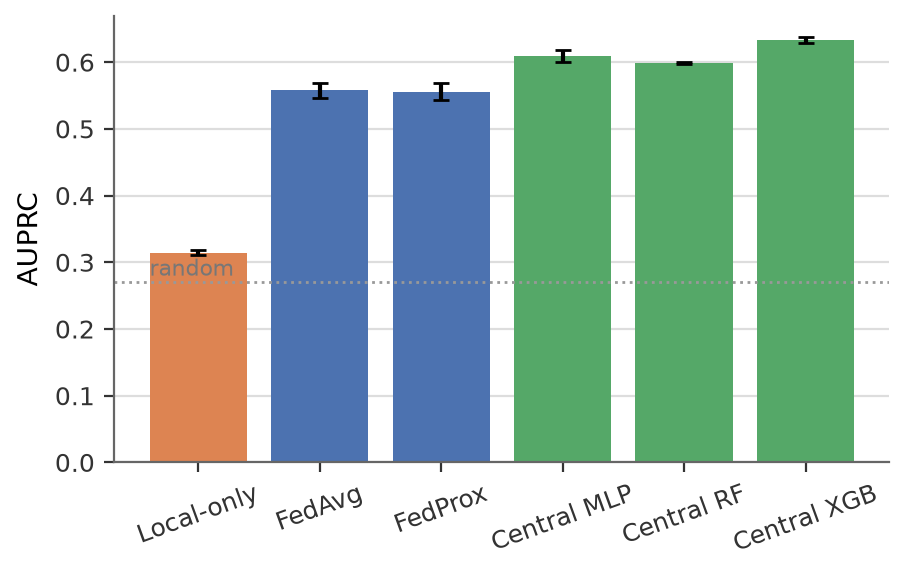
\includegraphics[width=0.8\textwidth]{main_results.png}
\caption{AUPRC by training regime, publisher partition (3 seeds).
Federation (blue) recovers most of the unattainable centralized ideal (green)
and far exceeds the silo-local status quo (orange).}
\label{fig:main}
\end{figure}

\begin{figure}[t]
\centering
\begin{minipage}[t]{0.48\textwidth}
\centering
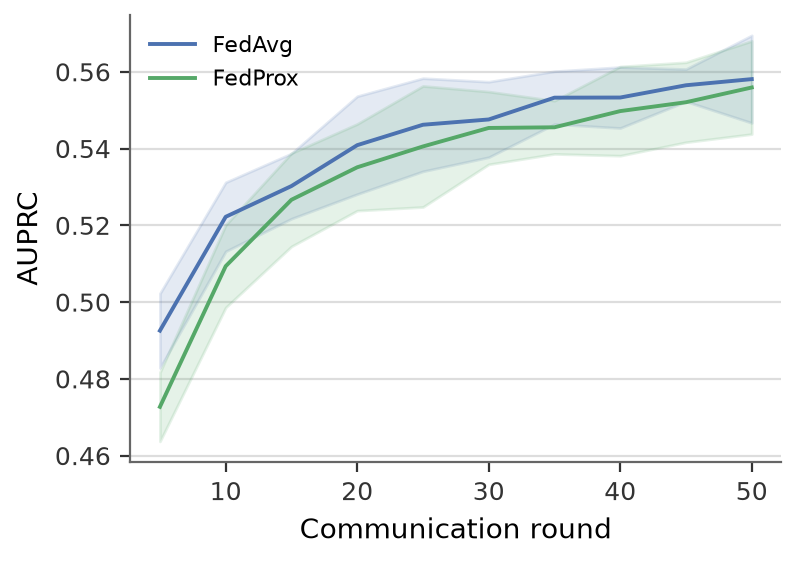
\includegraphics[width=\textwidth]{convergence.png}
\caption{Federated convergence over communication rounds (publisher silos).}
\label{fig:conv}
\end{minipage}\hfill
\begin{minipage}[t]{0.48\textwidth}
\centering
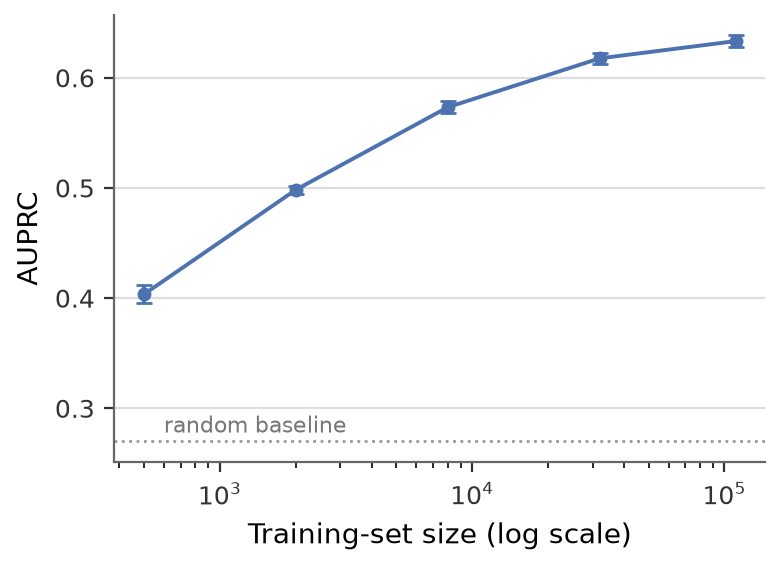
\includegraphics[width=\textwidth]{scale_curve.png}
\caption{Centralized AUPRC vs.\ training-set size: signal grows
monotonically with scale.}
\label{fig:scale}
\end{minipage}
\end{figure}

\subsection{Why scale matters}
Fig.~\ref{fig:scale} varies training-set size for the centralized XGBoost:
AUPRC rises monotonically from 0.403 (500 articles, the scale of prior
hand-curated corpora) through 0.573 (8K) to 0.633 (110K) and has not
saturated. Sub-thousand corpora forfeit more than a third of attainable
performance, an independent motivation for training at the scale only a
federation can reach.

\subsection{Feature families: accuracy vs.\ portability}
On the full corpus (Fig.~\ref{fig:ablation}), metadata features dominate
in-domain accuracy (AUPRC 0.593 alone vs.\ 0.381 for abstract linguistics
alone; 0.633 combined), and XGBoost feature importance concentrates on
citation dynamics (total citations 0.136, early citations 0.128), echoing the
citation-centric findings of~\cite{ref_usman_tpdl24}. The cross-corpus
experiments of Sect.~\ref{sec:transfer}, however, show the roles reverse
under domain shift: linguistic signal transfers, metadata does not.

\begin{figure}[t]
\centering
\begin{minipage}[t]{0.48\textwidth}
\centering
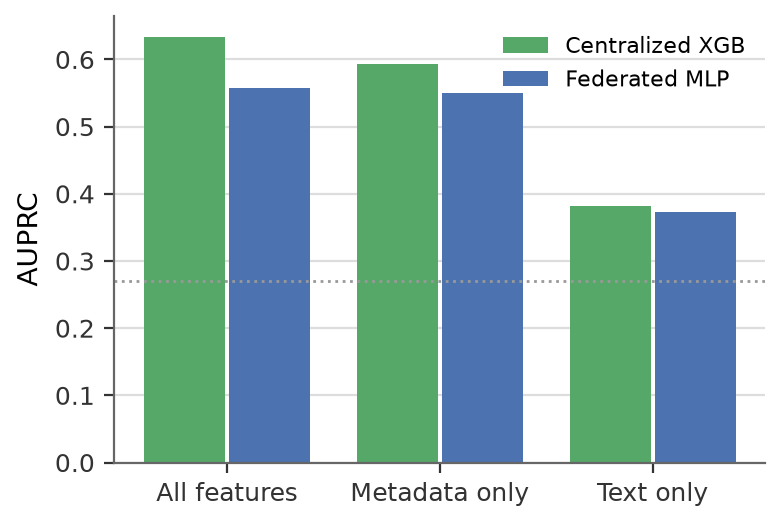
\includegraphics[width=\textwidth]{feature_ablation.png}
\caption{Feature-family ablation, centralized and federated.}
\label{fig:ablation}
\end{minipage}\hfill
\begin{minipage}[t]{0.48\textwidth}
\centering
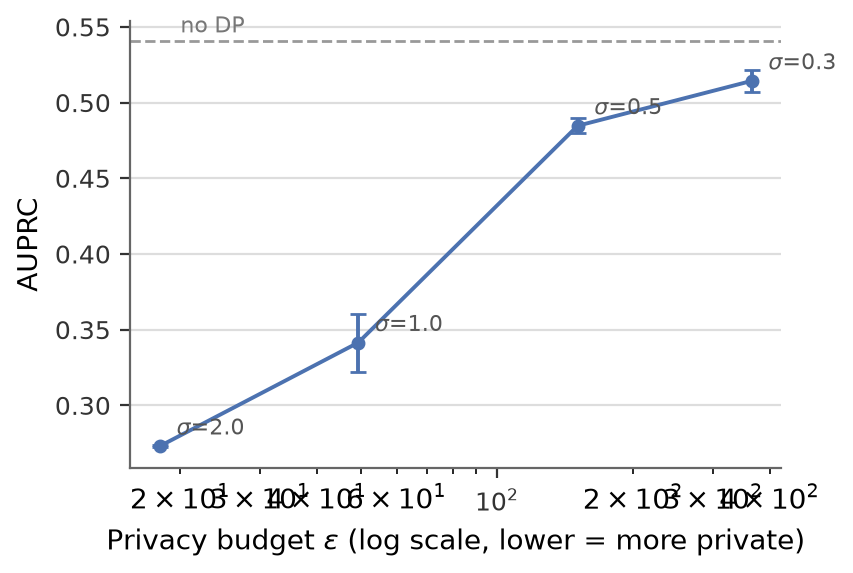
\includegraphics[width=\textwidth]{privacy_utility.png}
\caption{Privacy--utility trade-off of DP aggregation
(Algorithm~\ref{alg:fl}).}
\label{fig:dp}
\end{minipage}
\end{figure}

\subsection{Robustness: consortium size and temporal deployment}
\emph{Consortium size.} Varying the partition from $K{=}5$ to $K{=}20$
publisher silos changes FedAvg AUPRC only within noise
(0.574/0.558/0.560/0.558 for $K{=}5/10/15/20$): the federation does not
degrade as more, smaller publishers join.
\emph{Temporal split.} Training on articles published up to 2018 (52{,}506)
and testing on 2019 onward (86{,}031) is strictly harder for every regime
(centralized XGBoost 0.436, MLP 0.424), reflecting distribution drift and
retraction lag: many recent positives are not yet labeled. Critically,
the federated model keeps pace (0.407, i.e., 93\% of the centralized MLP
ratio), so the cost of federation does not grow under realistic prospective
deployment.

\subsection{Per-silo effects and fairness}
Evaluated on \emph{their own} test slices, large publishers' local models fit
their in-distribution data well (e.g., Elsevier 0.708 local vs.\ 0.578
federated), while data-poor or atypical silos gain from federation (PLOS
0.419 vs.\ 0.386; Spandidos 0.449 vs.\ 0.425); see Fig.~\ref{fig:persilo}.
Local specialization, however, is exactly what collapses on out-of-silo data
(Sect.~\ref{sec:main}: local-only 0.315 globally). The federation thus buys
universal coverage, benefits the weakest members most, and motivates
\emph{personalized} FL (a global backbone with silo-specific heads) as
future work.

\begin{figure}[t]
\centering
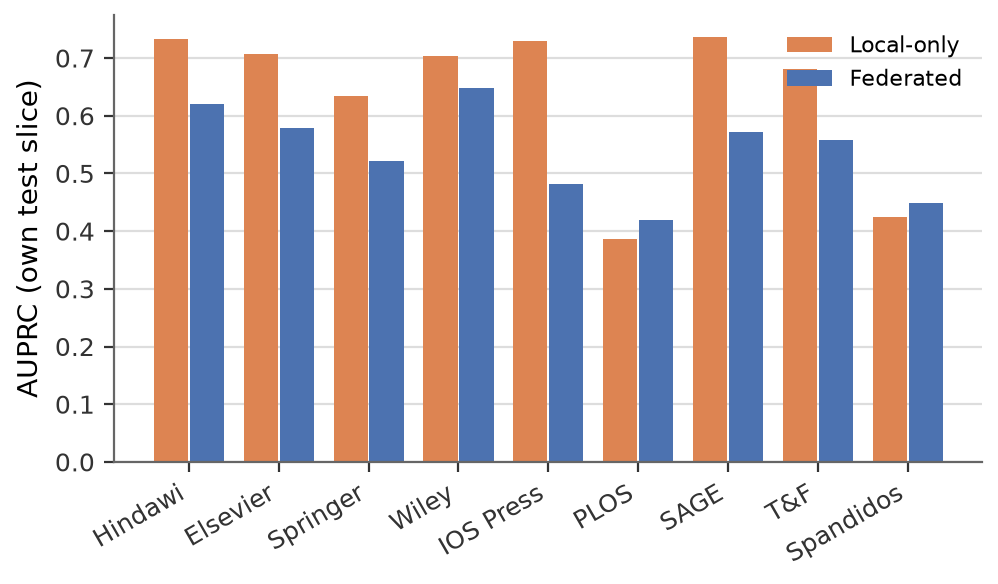
\includegraphics[width=0.8\textwidth]{per_silo.png}
\caption{Local vs.\ federated AUPRC on each publisher's own test slice.
Federation helps data-poor silos; large silos specialize locally but fail
globally (cf.\ Table~\ref{tab:main}).}
\label{fig:persilo}
\end{figure}

\subsection{Privacy--utility trade-off}
Fig.~\ref{fig:dp} sweeps the noise multiplier
$\sigma \in \{0.3, 0.5, 1.0, 2.0\}$ at clip $C{=}1$. Moderate noise
($\sigma{=}0.3$) retains 95\% of the non-private AUPRC (0.514 vs.\ 0.540);
$\sigma{\geq}1$ collapses utility. Because only $K{=}10$ clients participate,
the resulting formal $\varepsilon$ values are large; with realistic
consortium sizes (hundreds of publishers and journals) the same mechanism
yields far stronger guarantees. We report the curve as an honest
characterization of the mechanism at benchmark scale.

\subsection{Cross-corpus transfer against the hand-curated benchmark}
\label{sec:transfer}
We obtained the publicly released corpus of~\cite{ref_usman_websci25}
(232 retracted / 232 matched non-retracted biomedical articles with full-text
sections). Table~\ref{tab:transfer} reports three experiments that jointly
characterize the relationship between the small-corpus and large-corpus
regimes.

\begin{table}[t]
\centering
\caption{Cross-corpus experiments. Random AUPRC: 0.50 on the balanced
corpus of~\cite{ref_usman_websci25}, 0.27 on ours.}
\label{tab:transfer}
\small
\begin{tabular}{@{}lp{6.5cm}cc@{}}
\toprule
\# & Experiment & AUPRC & Baseline \\
\midrule
T1 & RF trained on 464 curated articles $\rightarrow$ our 138K corpus &
0.283 & 0.27 \\
T2 & Our federated model (all features) $\rightarrow$ curated corpus &
0.508 & 0.50 \\
T3 & Our model, \emph{linguistic features only} $\rightarrow$ curated corpus &
\textbf{0.691} & 0.50 \\
T4 & RF on curated corpus itself, abstract-only features (5-fold CV) &
0.525 & 0.50 \\
\bottomrule
\end{tabular}
\end{table}

Three findings follow. \emph{First} (T1), a model trained on hundreds of
curated articles collapses to chance on the open corpus: small-corpus results
do not generalize, independently of feature quality. \emph{Second} (T4),
restricted to abstract-level features, the very architecture that achieves
0.88 accuracy with full-text sections~\cite{ref_usman_websci25} drops to
chance on its own corpus; to our knowledge this is the first quantification of how
much retraction signal resides exclusively in paywalled full text. This is
the strongest empirical argument for federation: the decisive features exist
only where the data cannot leave. \emph{Third} (T2 vs.\ T3), our large-corpus
model transfers to the curated biomedical benchmark only through its
\emph{linguistic} features (0.691); adding metadata features destroys
transfer (0.508), since citation and era priors are domain-specific. Writing
style is the portable component of retraction signal.

\section{Discussion and Limitations}
\label{sec:discussion}
\emph{Simulation vs.\ deployment.} Our silos are simulated from public
metadata; a production federation would add per-publisher full-text
features, the signals T4 shows to be decisive, making our results a
conservative lower bound. \emph{Label noise.} Recent articles may be
retracted after data collection; the temporal experiment bounds this effect.
\emph{Coverage bias.} Retraction Watch over-represents fields and publishers
with active integrity teams; publisher-year matching removes the
corresponding shortcut from the classifier but not from the label
distribution. \emph{Privacy formalism.} With $K{=}10$ clients, DP guarantees
are loose; they tighten mechanically with consortium size. \emph{Negative
result.} A focal-loss, prevalence-weighted aggregation variant (FedBal,
Table~\ref{tab:main}) did not outperform FedAvg because matched controls
equalize prevalence across silos by construction; under unmatched deployment
prevalence skew it remains an open question.

\section{Conclusion}
\label{sec:conclusion}
We reformulated retraction prediction as cross-silo federated learning and
showed, on a corpus 180$\times$ larger than prior work, that publishers can
jointly train a screening model that recovers 92\% of the unattainable
centralized ideal without sharing a single record, while models trained on
any silo alone, or on small curated corpora, fail outside their origin. By
quantifying the full-text signal locked behind paywalls (0.88 $\rightarrow$
chance without it) and the portability of linguistic features, our results
chart the path to integrity screening at the scale of the scientific record:
a publisher federation, linguistically grounded features, and privacy
mechanisms whose guarantees strengthen exactly as the federation grows. For
the digital-library and scholarly-communication community, this reframes
retraction screening from a data-pooling problem, which is legally
foreclosed, into a model-sharing one, which is not.

\section*{Data availability}
The corpus is built from open sources: the Retraction Watch database
(distributed via Crossref), the OpenAlex API, and Europe PMC. The
corpus-construction pipeline, feature extraction, and all experiment
configurations are released to enable full reproduction (repository URL to be
inserted upon acceptance).

\section*{Declaration of competing interest}
The author declares no competing financial interests or personal
relationships that could have appeared to influence the work reported in this
paper.

\section*{Declaration of generative AI in the writing process}
The author used AI-assisted tools for language editing and LaTeX formatting.
All scientific content, experiments, analyses, and conclusions are the
author's own, and the author reviewed and takes full responsibility for the
content of the manuscript.

\begin{thebibliography}{99}
\bibitem{ref_rw}
Retraction Watch Database. Center for Scientific Integrity / Crossref (2023--2026).
\url{http://retractiondatabase.org}

\bibitem{ref_vannoorden}
Van Noorden, R.: More than 10,000 research papers were retracted in 2023 -- a
new record. Nature \textbf{624}, 479--481 (2023)

\bibitem{ref_usman_tpdl23}
Usman, M., Balke, W.-T.: On retraction cascade? Citation intention analysis as
a quality control mechanism in digital libraries. In: TPDL 2023, LNCS 14241,
pp. 117--131. Springer (2023)

\bibitem{ref_usman_tpdl24}
Usman, M., Balke, W.-T.: Tracing the retraction cascade: identifying
non-retracted but potentially retractable articles. In: TPDL 2024, LNCS,
pp. 109--126. Springer (2024)

\bibitem{ref_usman_dasfaa25}
Usman, M., Das, M., Balke, W.-T.: Anticipating retractions in scientific
databases using LLM-based citation analysis. In: DASFAA 2025. Springer (2025)

\bibitem{ref_usman_websci25}
Usman, M., Balke, W.-T.: Scientific accountability: detecting salient features
of retracted articles. In: Proc.\ 17th ACM Web Science Conference (WebSci
2025). ACM (2025)

\bibitem{ref_bibliometric}
Shi, X., et al.: Bibliometric feature identification and analysis of retracted
papers in biomedicine: an interpretable machine learning perspective. Inf.
Process. Manag. \textbf{62}(4) (2025)

\bibitem{ref_fedavg}
McMahan, B., Moore, E., Ramage, D., Hampson, S., Ag{\"u}era y Arcas, B.:
Communication-efficient learning of deep networks from decentralized data.
In: AISTATS 2017, pp. 1273--1282 (2017)

\bibitem{ref_fedprox}
Li, T., Sahu, A.K., Zaheer, M., Sanjabi, M., Talwalkar, A., Smith, V.:
Federated optimization in heterogeneous networks. In: MLSys 2020 (2020)

\bibitem{ref_kairouz}
Kairouz, P., McMahan, H.B., et al.: Advances and open problems in federated
learning. Found. Trends Mach. Learn. \textbf{14}(1--2), 1--210 (2021)

\bibitem{ref_dpfl}
McMahan, H.B., Ramage, D., Talwar, K., Zhang, L.: Learning differentially
private recurrent language models. In: ICLR 2018 (2018)

\bibitem{ref_openalex}
Priem, J., Piwowar, H., Orr, R.: OpenAlex: a fully-open index of scholarly
works, authors, venues, institutions, and concepts. arXiv:2205.01833 (2022)

\bibitem{ref_flesch}
Flesch, R.: A new readability yardstick. J. Appl. Psychol. \textbf{32}(3),
221--233 (1948)

\bibitem{ref_kincaid}
Kincaid, J.P., Fishburne, R.P., Rogers, R.L., Chissom, B.S.: Derivation of new
readability formulas for Navy enlisted personnel. Research Branch Report 8-75
(1975)
\end{thebibliography}

\end{document}
